\chapter{Konzept}\label{sec:concept}

Dieses Kapitel befasst sich mit der Entwicklung von Konzepten zur Bestimmung der Blickrichtung von Radfahrenden. Darüber hinaus wird diskutiert, wie eine ermittelte Blickrichtung genutzt werden kann, um eine Aussage darüber zu treffen, ob eine Person während der Fahrt auf das Display des Smartphones schaut.

Aufbauend auf den in Kapitel \ref{sec:related} vorgestellten verwandten Arbeiten wurden drei verschiedene Ansätze identifiziert. Diese werden in diesem Kapitel getestet und auf ihre Anwendbarkeit im Rahmen der PrioBike-App untersucht.

Dazu wird zunächst untersucht, ob Methoden zur Vorhersage von zweidimensionalen Bildschirmkoordinaten während der Fahrradfahrt eingesetzt werden können. 

Anschließend wird diskutiert, wie der Ansatz Henseler \cite{bachelor:henseler:gaze-ebikes}, die Blickrichtung anhand der Kopfrotation zu bestimmen, im Rahmen der PrioBike-App umgesetzt werden kann.  Schließlich wird ein Konzept vorgestellt, das auf Deep Learning Appearance-Based Methoden basiert, um die dreidimensionale Blickrichtung von Radfahrenden zu schätzen.

\section{Bestimmung der Blickrichtung anhand von zweidimensionalen Bildschirmkoordinaten}\label{sec:concept:2d}

Als erstes wurde untersucht, ob ein speziell für die Vorhersage von zweidimensionalen Bildschirmkoordinaten trainiertes Modell im Rahmen der PrioBike-App eingesetzt werden kann. Eine solches Verfahren ist vor allem für ruhende Personen vor einem Bildschirm optimiert. Eine große Variation der Kopfrotation oder Beleuchtung der Person ist dabei nicht zu erwarten, weshalb eine solche Methoden Schwierigkeiten bei einem Einsatz auf dem Fahrrad haben könnte. Vor allem aber muss eine solche Methode für den Anwendungsfall der PrioBike-App erkennen, zu welchen Zeitpunkten Radfahrende nicht auf ihr Smartphone sehen. 

Um dies zu untersuchen, wurde ein Prototyp entwickelt, der auf der Arbeit von Papoutsaki et al. \cite{paper:webgazer} basiert, die in Kapitel \ref{sec:related:webgazer} vorgestellt wurde. In dieser Arbeit stellen Papoutsaki et al. \textit{WebGazer} vor. Dabei handelt es sich um eine JavaScript-Bibliothek, die in jede Webseite eingebunden werden kann. \textit{WebGazer} ermöglicht die Vorhersage von Bildschirmkoordinaten auf der Grundlage des von einer Webcam aufgenommenen Bildes einer Person. Damit kann ein Ansatz entwickelt werden, der unabhängig vom Betriebssystem in einem Browser des Smartphones funktioniert, was für den Anwendungsfall der PrioBike-App ideal ist. \textit{WebGazer} benötigt weiterhin keine direkte Kalibrierung, sondern nutzt Benutzerinteraktionen wie Mausklicks und Mausbewegungen um die Blickrichtungsbestimmung während der Nutzung der Anwendung zu optimieren.

Der Prototyp wurde zunächst auf einem Laptop und einem Smartphone von einer ruhenden Person getestet, die frontal zu dem Bildschirm und der Kamera orientiert war. Die Person sollte dabei nur auf den Bildschirm schauen. Dazu wurde zuvor eine Kalibrierung durchgeführt, bei der die Person auf neun verschiedene Punkte schauen und klicken sollte. Die Qualität der Vorhersagen von \textit{WebGazer} wurde anschließend von der Testperson qualitativ bewertet. Die Vorhersagen wurden generell als gut eingeschätzt. Es wurde jedoch festgestellt, dass die Vorhersagen auf dem Smartphone etwas ungenauer waren. Außerdem wurde festgestellt, dass die Qualität unter schlechten Lichtverhältnissen, wie zum Beispiel in einem dunklen Raum oder bei einer Lichtquelle im Rücken der Person, sehr stark abnahm. Anschließend wurde der Prototyp noch einmal ohne vorherige Kalibrierung getestet, da solche Interaktionen mit der App während der Fahrt vermieden werden. Außerdem wäre eine Kalibrierung vor Fahrtbeginn wenig sinnvoll, da sich die Position der Personen auf dem Fahrrad während der Fahrt ändert. Die Ergebnisse waren auch bei diesem Versuch gut, allerdings schlechter als mit der Kalibrierung.

Anschließend sollte überprüft werden, wie gut mit einem solchen Ansatz erkannt wird, ob die Person auf den Bildschirm sieht oder nicht. Dafür wird angenommen, dass \textit{WebGazer} in einem solchen Fall entweder tatsächlich die Koordinaten des absoluten Bildschirmrandes vorhersagt oder zumindest Koordinaten in der Nähe des Bildschirmrandes. Deshalb wurde eine Zone am Rand des Bildschirms definiert. Dieser Bereich ist in der Abbildung \ref{fig:concept:webgazer:threshold} blau markiert. Liegt die Vorhersage in diesem Bereich, wird davon ausgegangen, dass die Person nicht auf das Gerät schaut.

\begin{figure}
    \centering
    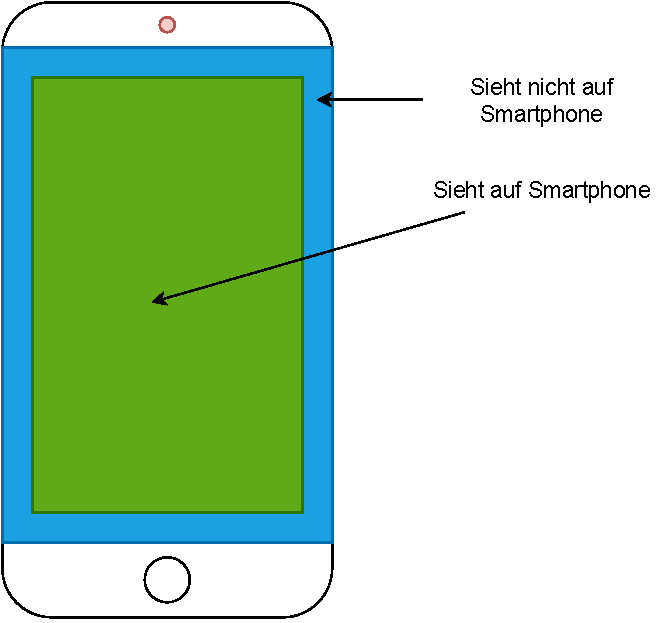
\includegraphics[width=0.5\linewidth]{concept/webgazer.drawio.pdf}
    \caption{Darstellung des Grenzwertes am Rand des Smartphones (blau). Fällt die Prognose in diese Zone, soll angenommen werden, dass die Person nicht auf das Smartphone sieht.}
    \label{fig:concept:webgazer:threshold}
\end{figure}

Doch bereits die ersten Tests mit dem neuen Prototypen haben gezeigt, dass dieser Ansatz bereits bei einem Laptop mit einem größeren Bildschirm als bei einem Smartphone nicht funktioniert. Wenn absichtlich nicht auf den Bildschirm gesehen wurde, waren die Vorhersagen sehr ungenau. Sie wurden nicht wie erwartet am Rand des Bildschirms angezeigt. Beispiele für solche Fehlerfälle sind in der Abbildung \ref{fig:concept:webgazer:wrong} zu sehen. Dasselbe Verhalten konnte bei dem Einsatz auf einem Smartphone beobachtet werden. 

\begin{figure}{}
    \begin{subfigure}{0.9\textwidth}
        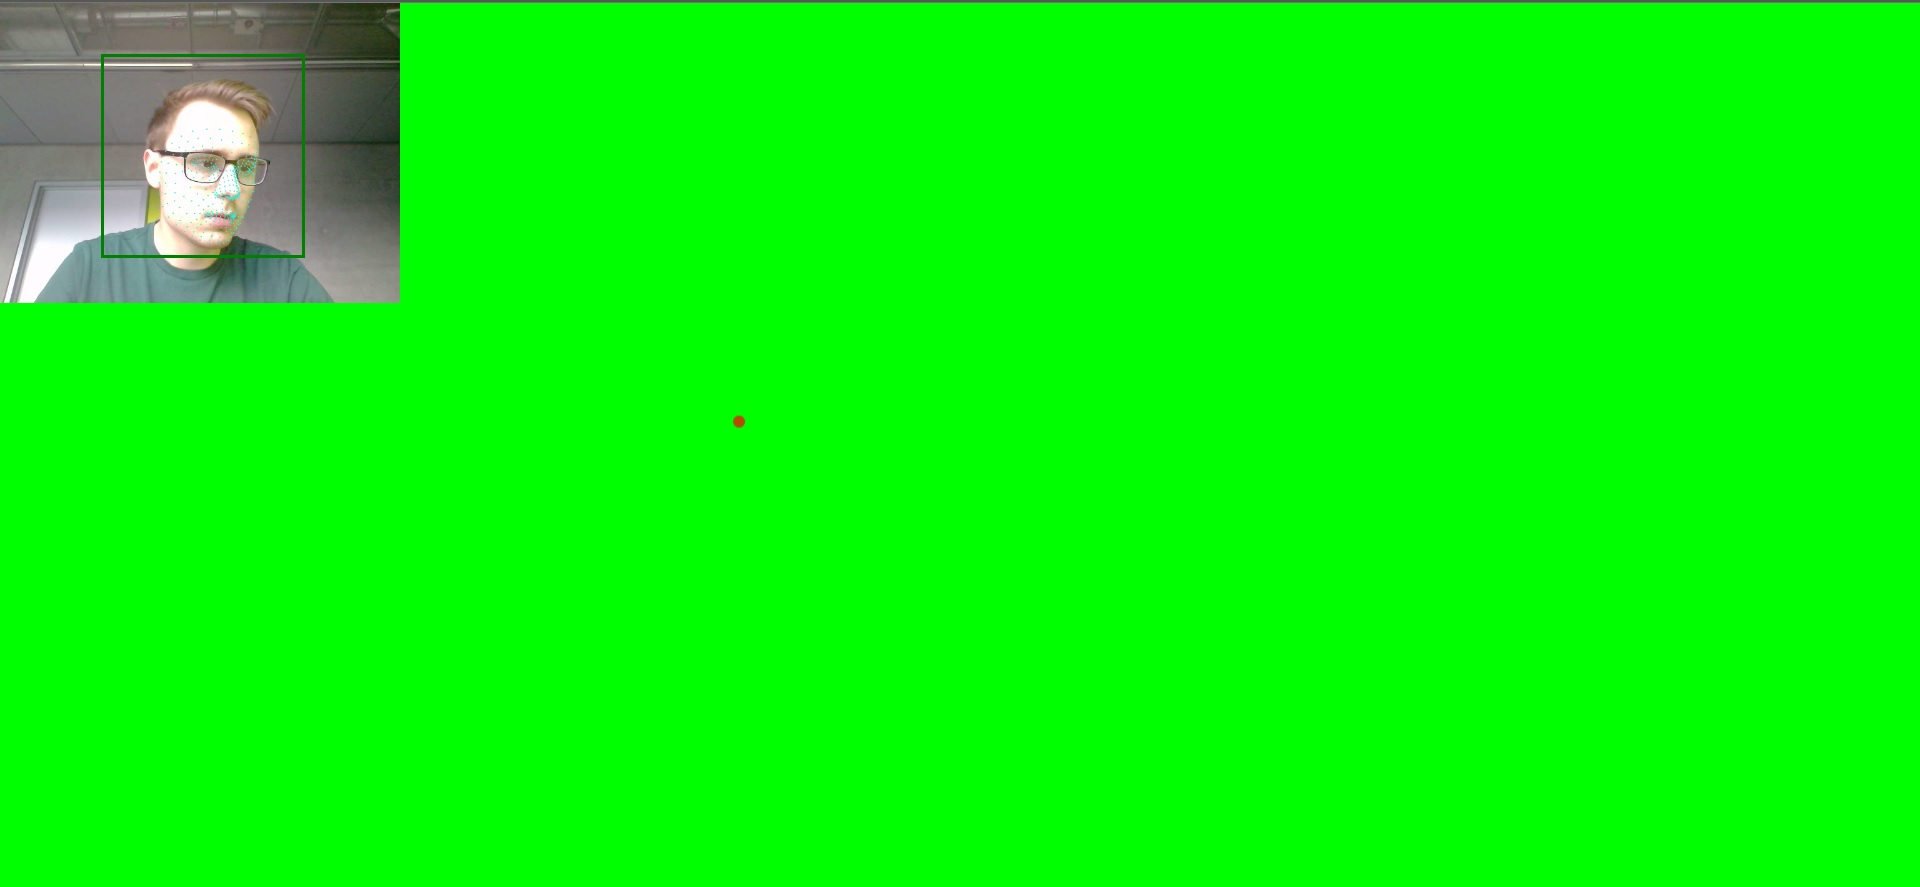
\includegraphics[width=\linewidth]{webgazer/webgazer_wrong_1.jpg}
    \end{subfigure}%
     \vspace{0.5cm} % Abstand zwischen den beiden Bildern
    \begin{subfigure}{0.9\textwidth}
        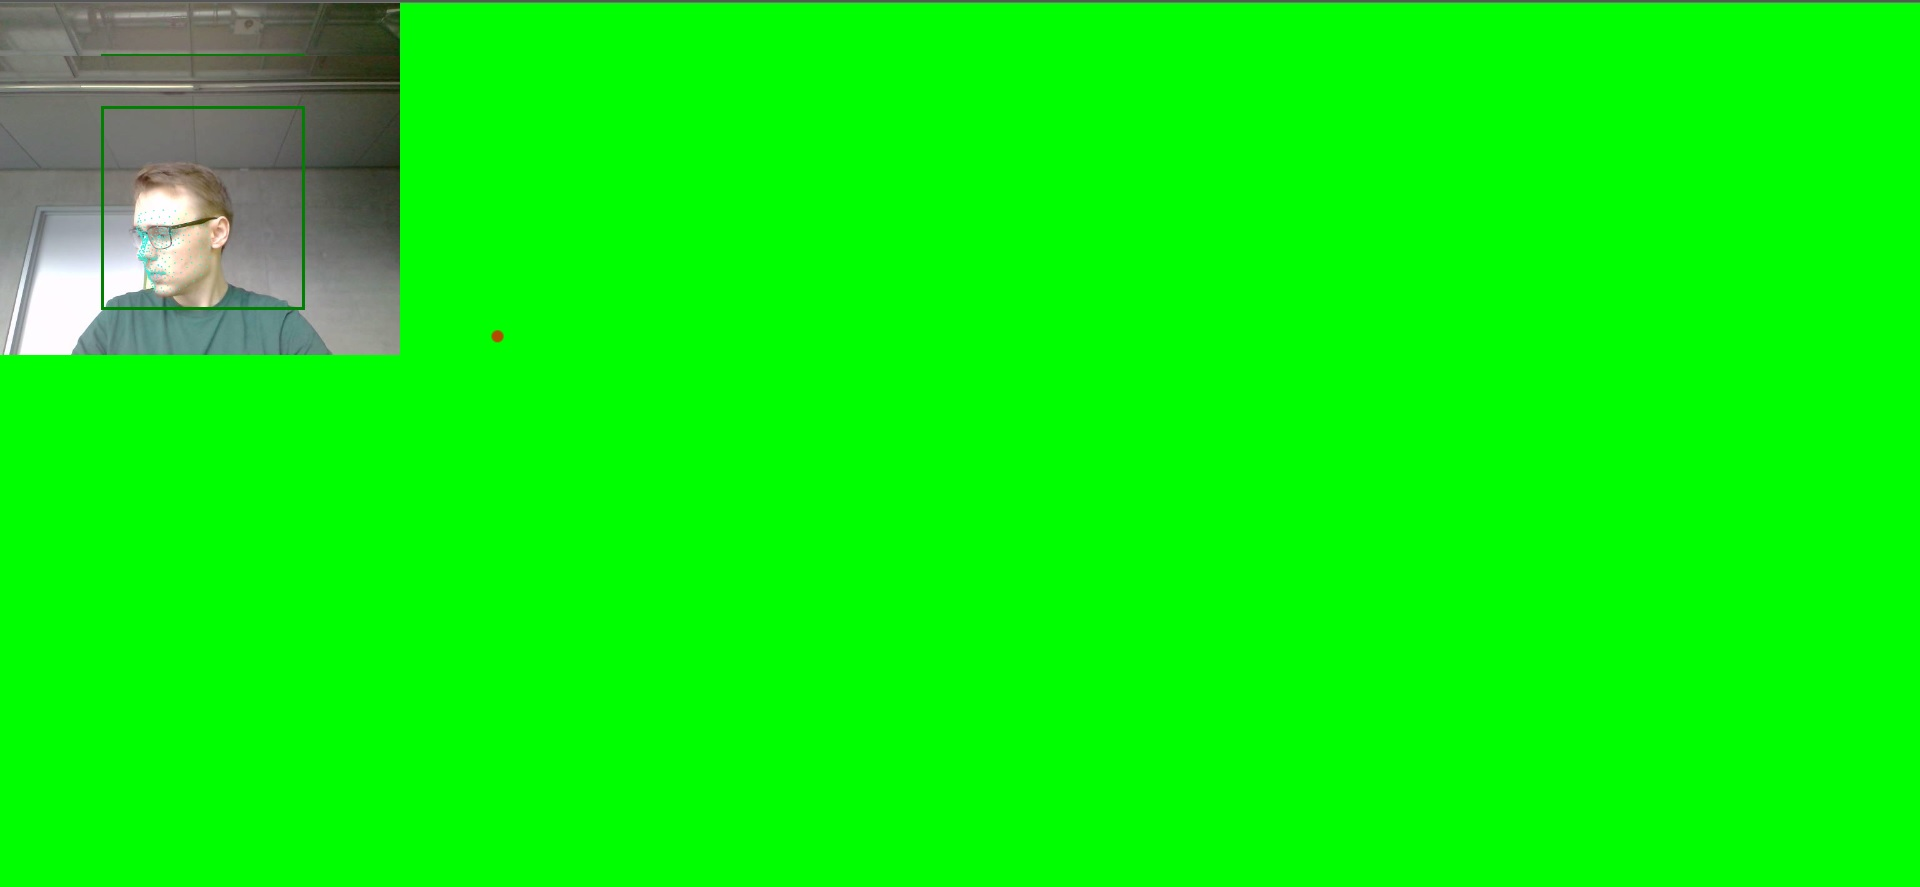
\includegraphics[width=\linewidth]{webgazer/webgazer_wrong_2.jpg}
    \end{subfigure}
    \caption{Beispiele für die Vorhersagen von WebGazer (roter Punkt), wenn eine Person nicht auf den Bildschirm sieht.}
    \label{fig:concept:webgazer:wrong}
\end{figure}

Somit kann mittels \textit{WebGazer} keine Aussage darüber getroffen werden, ob die Person auf das Smartphone schaut oder nicht. Daher ist ein solcher Ansatz für den Einsatz im Rahmen der PrioBike-App nicht geeignet, weshalb dieser Ansatz verworfen wurde. 

\section{Blickrichtungsbestimmung anhand der Kopfrotation}\label{sec:concept:head}

Ein weiterer in der Recherche identifizierter Ansatz besteht darin, die Blickrichtung von Radfahrenden anhand ihrer Kopfrotation zu bestimmen. Dieser Ansatz wird in der Arbeit von Henseler \cite{bachelor:henseler:gaze-ebikes} vorgestellt und in Kapitel \ref{sec:related:henseler} erläutert. Der Ansatz kann in mehrere Teilprobleme unterteilt werden. Zunächst muss das Gesicht des Radfahrenden im Bild erkannt werden. Anschließend müssen die Gesichtsmerkmale identifiziert werden. Abschließend erfolgt die Bestimmung der Kopfrotation anhand der erkannten Gesichtsmerkmale und eine Interpretation der Ergebnisse.  Die Umsetzung des von Henseler vorgestellten Ansatzes weist jedoch einige Probleme auf, die diese für den Einsatz im Rahmen der PrioBike-App ungeeignet machen. Die Umsetzung ist bezüglich der Lichtverhältnisse im Video sehr unflexibel. Zudem sind eine spezielle Smartphone-Halterung und eine Markierung am Fahrradhelm erforderlich. Außerdem treten die größten Ungenauigkeiten bei Henseler's Umsetzung auf, wenn es darum geht zu erkennen, wann die Person auf das Smartphone schaut.

Daher wurde untersucht, wie die Blickrichtung der Radfahrenden anhand der Kopfrotation robuster bestimmt werden kann. Es wurde festgestellt, dass das Thema der Gesichtserkennung und Gesichtsmerkmalsbestimmung in vielen verschiedenen Anwendungsbereichen von Bedeutung ist und daher bereits umfangreiche Forschung zu diesem Thema betrieben wurde, wie in Kapitel \ref{sec:related:face} erläutert wird. Dementsprechend gibt es auch einige Technologien, welche dafür entwickelt wurden, das Erkennen von Gesichtern und Gesichtsmerkmalen in Bildern zu ermöglichen. Um zu prüfen, ob diese Form der Gesichtserkennung für den Anwendungsfall der PrioBike-App geeignet ist, wurde ein Prototyp unter Verwendung von \textit{Google ML Kit}\footnote{\url{https://pub.dev/packages/google_ml_kit} (Abgerufen am 09.11.2023)} entwickelt. Diese Bibliothek wurde speziell für die Verwendung auf Smartphones entwickelt und ermöglicht das Lösen verschiedener Computer Vision Aufgaben mithilfe von maschinellem Lernen. So können mit \textit{Google ML Kit} Gesichter sowie eine Liste von Gesichtsmerkmalen in Form von zweidimensionalen Punkten erkannt werden. Ein Beispiel für das Ergebnis der Erkennung ist in Abbildung \ref{fig:concept:google_ml_kit} dargestellt.

\begin{figure}
    \centering
    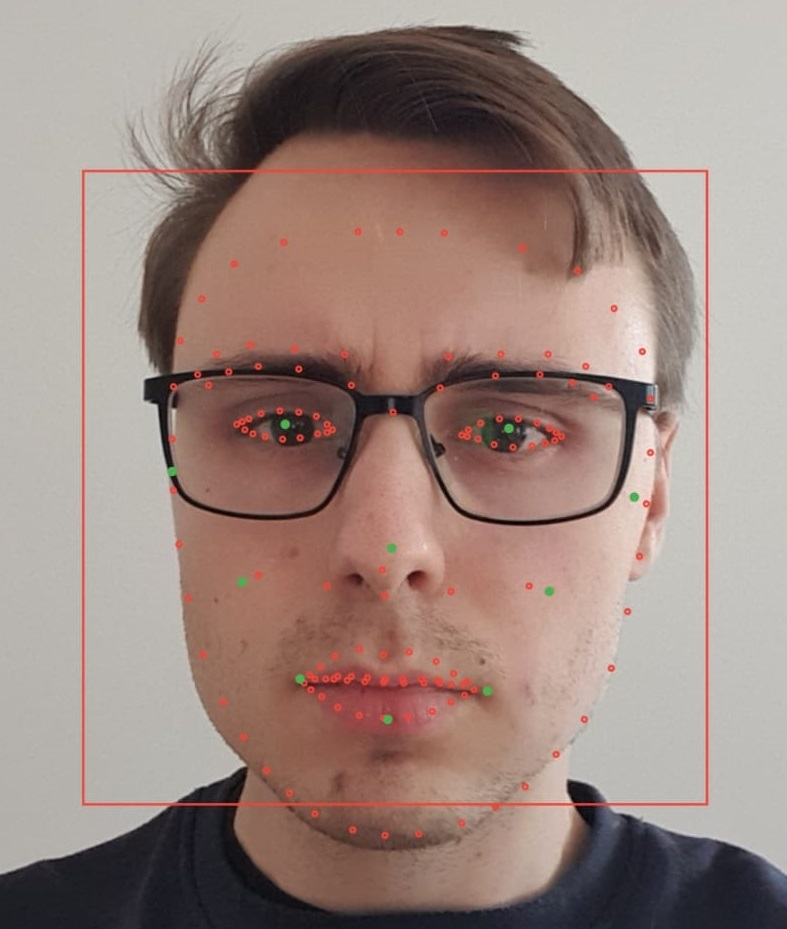
\includegraphics[width=0.5\linewidth]{concept/google_ml_kit.jpg}
    \caption{Erkannte Orientierungspunkte des Gesichts mit \textit{Google ML Kit}}
    \label{fig:concept:google_ml_kit}
\end{figure}

Mit diesem Prototypen wurden erste Tests durchgeführt, um den Einfluss von Licht, teilweise verdeckten Gesichtern und extremen Kopfrotationen auf die Qualität der Gesichtserkennung zu untersuchen. Es wurde festgestellt, dass die Erkennung auch bei sehr heller oder sehr dunkler Beleuchtung gut funktioniert. Es wurde auch kein Unterschied zwischen Personen mit und ohne Brillen festgestellt. Allerdings wurde beobachtet, dass die Qualität bei extremen Kopfrotationen, insbesondere entlang der Querachse, leicht nachgelassen hat. Insgesamt wurde dieser Ansatz der Gesichtserkennung jedoch als vielversprechend eingestuft.

\subsection{Betrachtung anhand Kopfrotation}

Nach der Erkennung der Gesichtsmerkmalen hat sich Henseler als nächstes mit der Bestimmung und Interpretation der Kopfrotation beschäftigt. Auch für dieses Problem bietet das \textit{Google ML Kit} eine Lösung, bei der anhand der erkannten Gesichtsmerkmale die Rotationswinkel entlang der Quer-, Längs- und Vertikalachse bestimmt werden können. Anhand dieser Werte soll nun entschieden werden, ob das Gesicht zum Smartphone orientiert ist oder nicht.

Dafür wurde der Prototyp weiterentwickelt. Es wurden experimentell Grenzwerte für die Rotationswinkel entlang der Quer- und Vertikalachse festgelegt. Wenn die erkannte Rotation bei einer der Achsen außerhalb dieser Grenzwerte liegt, wird davon ausgegangen, dass die dargestellte Person nicht auf das Smartphone schaut. Die Längsachse wurde dabei nicht berücksichtigt, da durch eine Rotation um diese Achse die generelle Orientierung des Gesichts zum Bildschirm unverändert bleibt. 

Dieser Ansatz hat gute Resultate bei einer ruhenden Person vor dem Bildschirm erzielt. Eine solche Person ist in der Abbildung \ref{fig:concept:google_vision:position:middle} zu sehen. Der Ansatz funktioniert jedoch nur, solange die Position des Kopfes im Bild konstant bleibt. In Abbildung \ref{fig:concept:google_vision:position:top} ist eine Person mit ähnlicher Kopfrotation wie in Abbildung \ref{fig:concept:google_vision:position:middle} zu sehen, allerdings ist zu erkennen, dass diese Person nicht auf das Smartphone sieht. Das zeigt, dass die ermittelten Grenzwerte von der Position und Größe des Kopfes im Bild abhängen. Aus diesem Grund müssten diese Grenzwerte je nach Position des Kopfes relativ zu Kamera angepasst und optimiert werden, da auf dem Fahrrad nicht gewährleistet werden kann, dass sich der Kopf immer in derselben Position im Bild befindet. Es muss daher eine andere Lösung gefunden werde, um die Kopfrotation zu interpretieren.

\begin{figure}[]
    \begin{subfigure}{0.35\textwidth}
        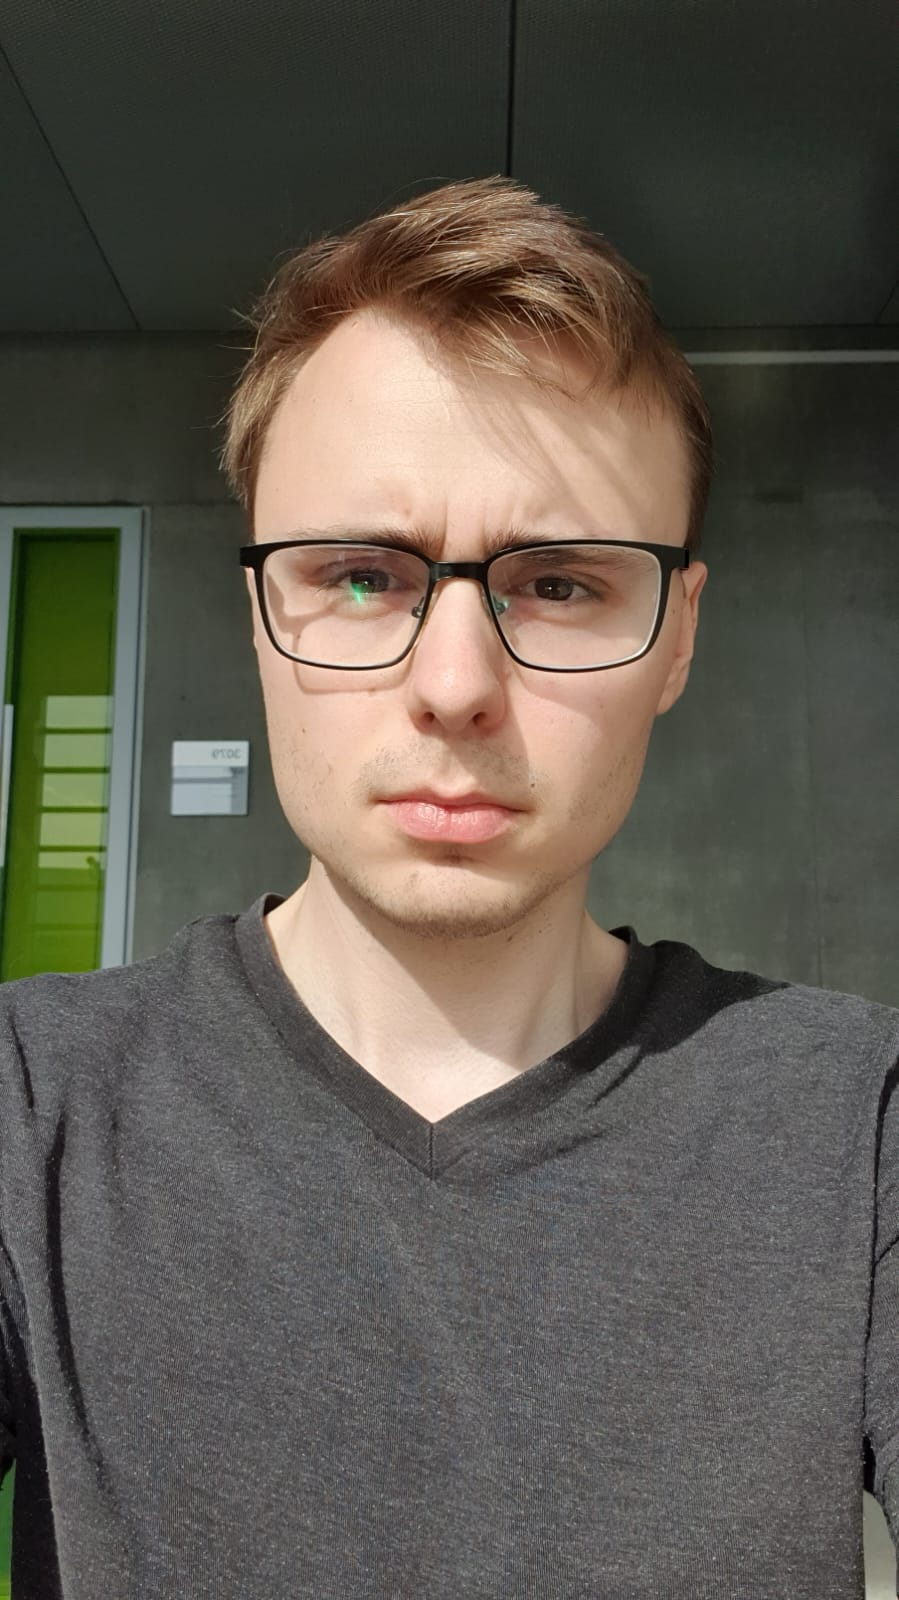
\includegraphics[width=\linewidth]{concept/googlevision/google_vision_schaut.jpg}
        \caption{Nutzer schaut auf das Smartphone-Display}
        \label{fig:concept:google_vision:position:middle}
    \end{subfigure}\hspace{0.5cm}
    \begin{subfigure}{0.35\textwidth}
        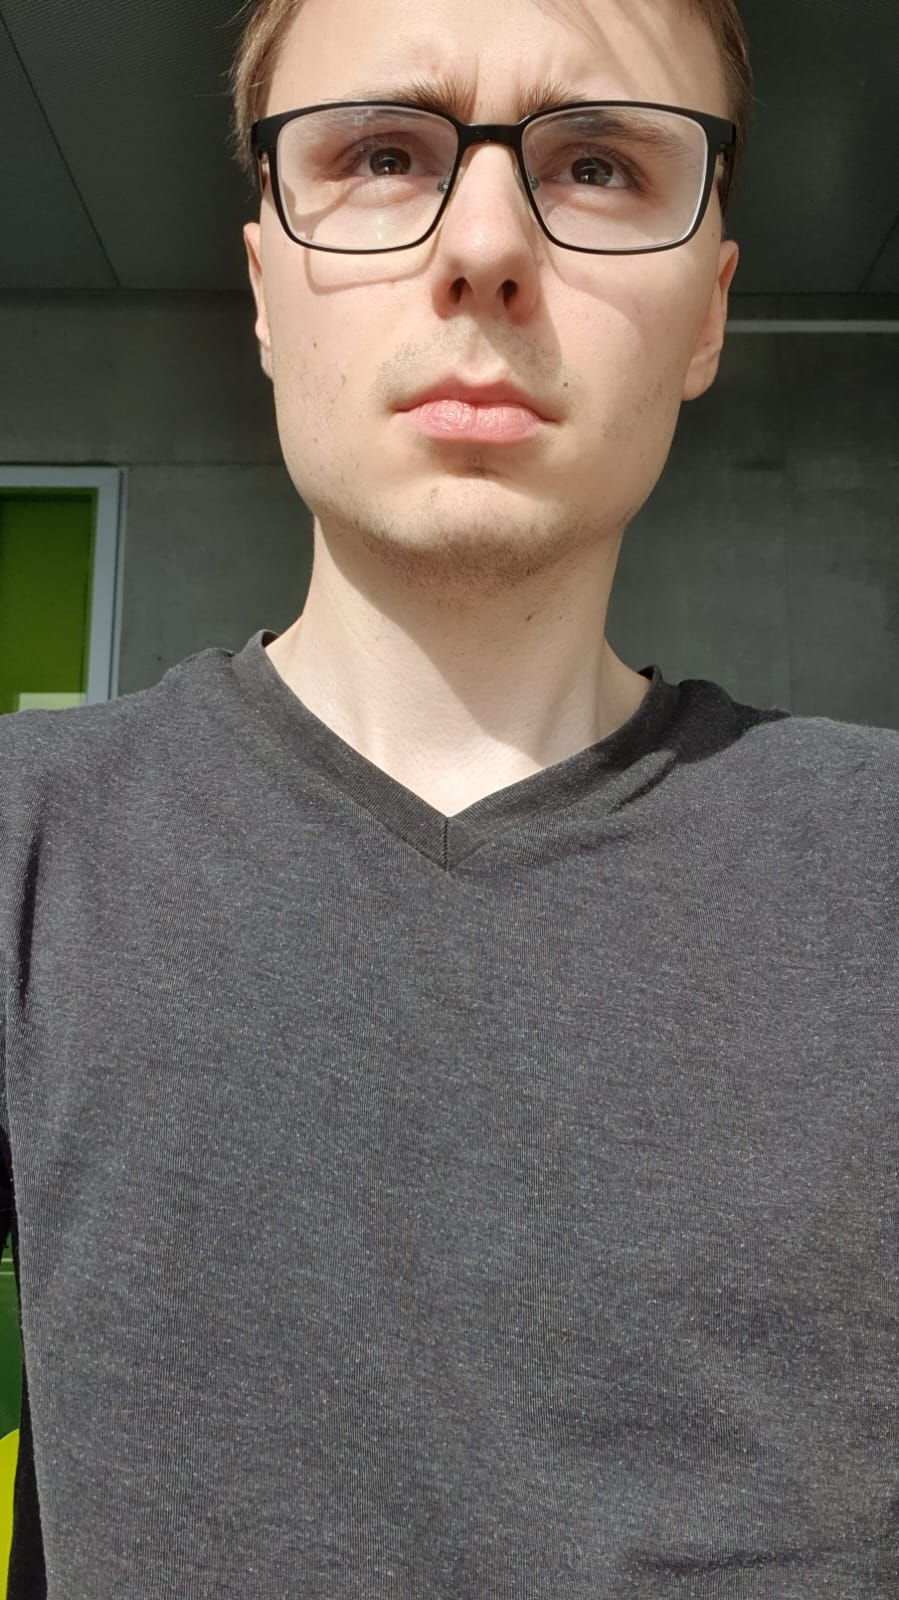
\includegraphics[width=\linewidth]{concept/googlevision/google_vision_schaut_nicht.jpg}
        \caption{Nutzer schaut nicht auf das Smartphone-Display}
        \label{fig:concept:google_vision:position:top}
    \end{subfigure}
    \caption{Darstellung der Auswirkung unterschiedlicher Kopfpositionen im Bild auf die Bedeutung der Kopfdrehung. Zweimal ist eine Person zu sehen, die fast keine Kopfdrehung aufweist. In Abbildung \ref{fig:concept:google_vision:position:middle} ist zu sehen, dass dies bedeutet, dass die Person auf das Smartphone schaut. In Abbildung \ref{fig:concept:google_vision:position:top} ist dieselbe Person mit derselben Kopfdrehung zu sehen. Es ist jedoch zu erkennen, dass die Person in diesem Bild nicht auf das Smartphone schaut.}
    \label{fig:concept:google_vision:position}
\end{figure}

\subsection{Dreidimensionale Betrachtung}\label{sec:concept:head:3d}

In einem neuen Ansatz wird die Entscheidung, ob eine Person auf das Smartphone schaut oder nicht, als dreidimensionales Problem betrachtet. Das Koordinatensystem des dreidimensionale Raumes wird dabei so konzipiert, dass die Kamera den Koordinatenursprung darstellt. Unter der Annahme, dass sich die Kamera in der Mitte des Bildes befindet, lässt sich die Position des Kopfes relativ zur Kamera anhand der zweidimensionalen Gesichtspunkte durch die x-Achse in der Breite und die y-Achse in der Höhe bestimmen. Allerdings ist die Tiefe $z$ dieser Punkte nicht bekannt. Da diese Gesichtspunkte im Sichtfeld der Kamera liegen, muss ihre Tiefe größer als null sein. Die Kamera liegt auf der dreidimensionalen Ebene $\cameraplane$, die durch $z = 0$ beschrieben werden kann. Da die Kamera fest im Smartphone integriert ist, hat auch das gesamte Display eine Tiefe von 0 und befindet sich damit ebenfalls auf derselben Ebene.
Wenn man annimmt, dass man die dreidimensionale Position eines Kopfes kennt, der sich direkt frontal vor der Kamera befindet und in keiner der Achsen rotiert wurde, kann man einen Richtungsvektor $\gazevector$ bestimmen, der parallel zur z-Achse und in Richtung der Ebene $\cameraplane$ verläuft. Dieser Richtungsvektor entspricht in diesem Fall der Blickrichtung des Kopfes. Mithilfe eines Punktes $\centerface$ des Kopfes und diesem Vektor $\gazevector$ lässt sich eine Gerade $G$ definieren, die orthogonal zur Ebene $\cameraplane$ verläuft und sie im Punkt $\intersection$ schneidet. 

Rotiert man diesen Kopf und entsprechend auch den Vektor $\gazevector$, dann verändert sich die Position des Schnittpunkts $\intersection$ auf der Ebene $\cameraplane$. Da das Display des Smartphones, wie bereits erwähnt, ebenfalls auf der Ebene $\cameraplane$ liegt, soll auf dieser Ebene $\cameraplane$ eine Zone definiert werden, die das Display des Smartphones repräsentiert. Wenn sich der Punkt $\intersection$ innerhalb dieser Zone befindet, sieht die dargestellte Person auf das Smartphone (siehe Abbildung \ref{fig:concept:head:example:yes}). Wenn sich der Punkt $\intersection$ außerhalb dieser Zone befindet, sieht die Person nicht auf das Smartphone (siehe Abbildung \ref{fig:concept:head:example:no}).

\begin{figure}[]
    \begin{subfigure}{0.8\textwidth}
        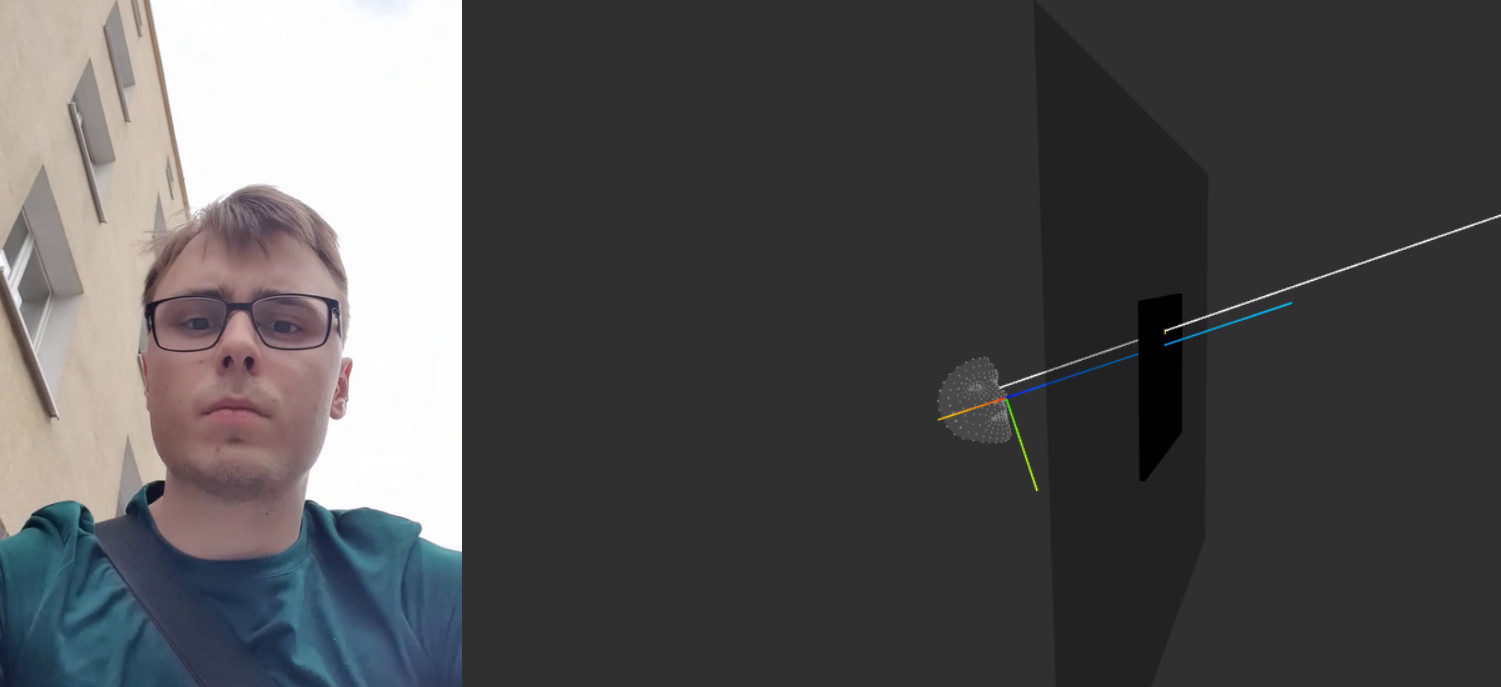
\includegraphics[width=\linewidth]{concept/concept_head_sieht.jpg}
        \caption{Person sieht auf Smartphone}
        \label{fig:concept:head:example:yes}
    \end{subfigure}
    \begin{subfigure}{0.8\textwidth}
        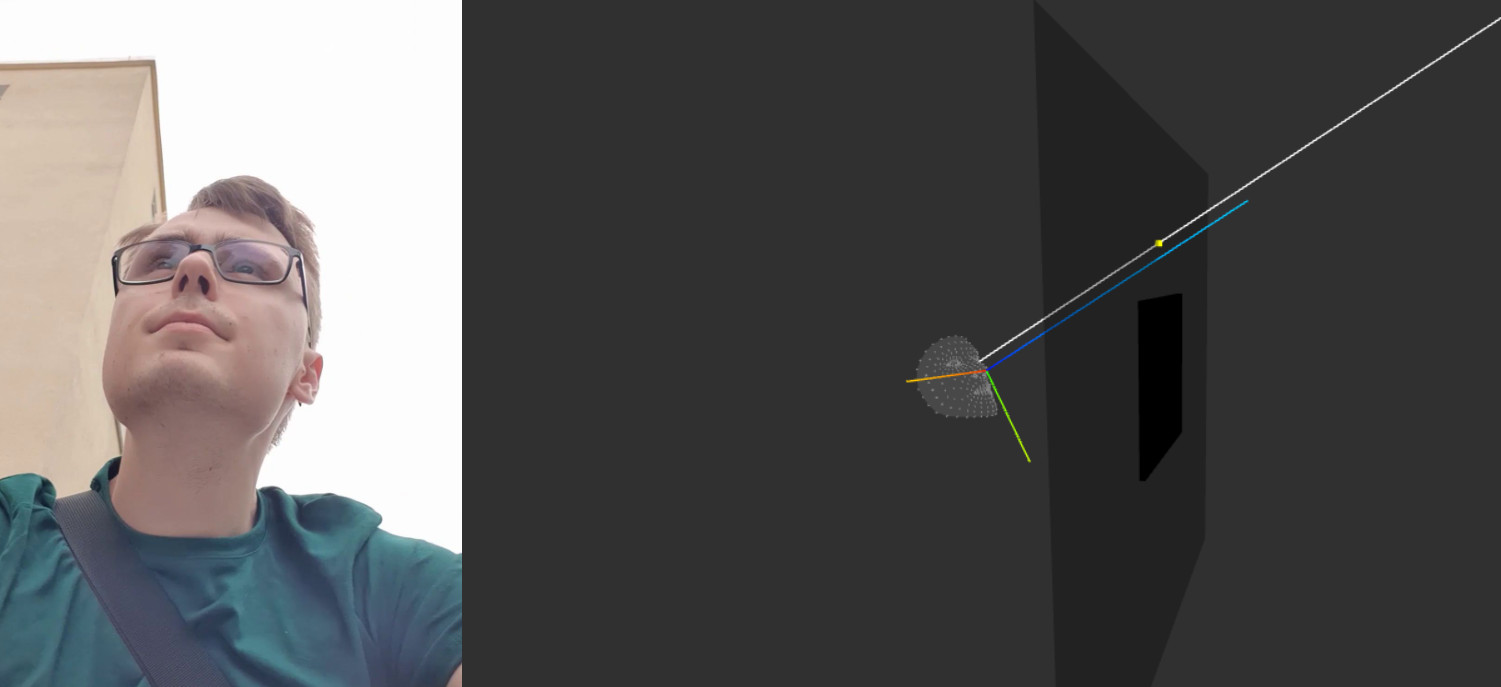
\includegraphics[width=\linewidth]{concept/concept_head_sieht_nicht.jpg}
        \caption{Person sieht nicht auf Smartphone}
        \label{fig:concept:head:example:no}
    \end{subfigure}
    \caption{Darstellung der dreidimensionalen Gesichtspunkte, der Ebene $\cameraplane$, der Geraden $G$, des Bereichs, der das virtuelle Smartphone-Display darstellt, und des entsprechenden Schnittpunkts $\intersection$.}
    \label{fig:concept:head:example}
\end{figure}

Über die Tiefe der einzelnen Gesichtspunkte gibt \textit{Google ML Kit} leider keine Aussage. Da der Abstand zwischen dem Kopf des Radfahrers je nach Körpergröße, Sitzhaltung und Fahrradtyp unterschiedlich ist, kann auch keine generelle Distanz geschätzt werden. 

Das Problem der Abbildung von zweidimensionalen Bildpunkten auf dreidimensionale Punkte wird als \textit{Pose Computation Problem} \cite{paper:pose:problem} bezeichnet. Dieses Problem wird unter anderem in der Arbeit von Zhang et al. über den \textit{ETH-XGaze} Datensatz diskutiert \cite{paper:eth-xgaze}. Zur Lösung dieses Problems nutzen sie ein spezielles dreidimensionales Modelle des Gesichts, das aus der gleichen Anzahl von Punkten bestehen wie die Anzahl der erkannten Gesichtsmerkmale. Zudem wird eine Abbildung verwendet, um zu ermitteln, welcher zweidimensionale Punkt zu welchem dreidimensionalen Punkt gehört. Anhand von diesem Modell lässt sich ein Rotationsvektor $\vec{r}$ und ein Translationsvektor $\vec{t}$ bestimmen. Diese geben an, wie das dreidimensionale Modell des Gesichts verformt und verschoben werden muss, um der durch die zweidimensionalen Bildpunkte gegeben Kopfposition zu entsprechen. Somit lässt sich aus den erkannten zweidimensionalen Punkten eine dreidimensionale Darstellung des Kopfes entwickeln, mit der der oben beschriebene Ansatz umgesetzt werden kann.

Auf dieser Grundlage wurde das erste Konzept für die Bestimmung der Blickrichtung in dieser Arbeit festgelegt. Hierfür sollen Videos von Radfahrenden mittels der Innenkamera des Smartphones unter verschiedenen Umweltbedingungen aufgenommen werden. Anschließend soll das Gesicht in den einzelnen Frames der Videos erkannt werden. Dafür sollen verschiedene Methoden zur Erkennung von Gesichtsmerkmalen verwendet werden, die in Kapitel \ref{sec:related:face} vorgestellt wurden. Mittels der dabei erkannten Gesichtspunkte soll im nächsten Schritt ein dreidimensionales Modell erstellt werden, mit dessen Hilfe dann die Gerade $G$ bestimmt wird, um den Schnittpunkt $\intersection$ mit der Ebene $\cameraplane$ zu finden. Anschließend soll untersucht werden, bei welchen dieser Schnittpunkte die Person auf das Smartphone gesehen hat, um so die beschriebene Zone auf der Ebene $\cameraplane$ zu bestimmen.

Um mögliche Fehlerquellen und Schwächen dieses Ansatzes zu untersuchen, soll die Erkennungsqualität der Gesichtsmerkmale evaluiert werden. Für eine quantitative Evaluation der erkannten Gesichtspunkte müssten für jedes aufgenommene Bild alle vorhandenen Gesichtspunkte manuell markiert werden \cite{paper:face:survey}. Leider ist dies im zeitlichen Rahmen dieser Arbeit nicht umsetzbar. Die Qualität der Gesichtserkennung soll daher subjektiv für jedes einzelne Bild eingeschätzt werden, was jedoch ebenfalls mit großem zeitlichem Aufwand verbunden ist. Aus diesem Grund können nicht alle in Kapitel \ref{sec:related:face} präsentierten Algorithmen in dieser Arbeit getestet werden.

Es wurde daher beschlossen, sich in erster Linie auf Gesichtserkennungsmethoden zu konzentrieren, die gut auf Smartphones genutzt werden können. Die Entscheidung fiel auf die Verwendung des \textit{Ensemble of Regression Trees (ERT)} und der Gesichtserkennungspipeline des \textit{MediaPipe} Frameworks. Diese Wahl wurde aufgrund der hohen Geschwindigkeit der Methoden und der Verfügbarkeit von Open-Source-Implementierungen getroffen.

Problematisch an diesem Ansatz ist, dass er darauf beruht, dass ein Gesicht und die entsprechenden Gesichtsmerkmale erkannt werden konnten. Daher stellt sich die Frage, ob eine Aussage darüber getroffen werden kann, ob die Person auf das Smartphone schaut oder nicht, obwohl kein Gesicht erkannt wurde. Wie bereits erwähnt, haben erste Tests mit dem Prototypen basierend auf \textit{Google ML Kit} gezeigt, dass vor allem eine starke Kopfdrehung zu Problemen bei der Gesichtserkennung geführt hat. Daher wird die Annahme getroffen, dass in den meisten Situationen, in welchen das Gesicht nicht identifiziert werden kann, dies auf die Rotation des Kopfes zurückzuführen ist. Weiter wird angenommen, dass wenn der Kopf extrem gedreht ist, sich das Smartphone am Lenker außerhalb des Blickfeldes der Person befindet und diese daher höchstwahrscheinlich nicht auf das Gerät schaut. Diese Annahme soll bei der Evaluation des Ansatzes untersucht werden. Wenn diese Annahme bestätigt werden kann, kann gesagt werden, dass wenn kein Gesicht erkannt wurde, die Person auch höchstwahrscheinlich nicht auf das Smartphone gesehen hat.

\subsection{MediaPipe}

Das in Kapitel \ref{sec:concept:head:3d} beschriebene Konzept basiert ausschließlich auf der Rotation und Position des Kopfes. Der große Nachteil dieses Ansatzes ist jedoch, dass die Blickrichtung der Augen nicht berücksichtigt wird, die das Ergebnis der Vorhersage noch weiter verfeinern könnte. Bei der Recherche wurde das Framework \textit{MediaPipe} \cite{paper:mediapipe} entdeckt, welches in Kapitel \ref{sec:related:mediapipe} vorgestellt wurde. Teil des Frameworks ist die \textit{FaceLandmarker}\footnote{\url{https://developers.google.com/mediapipe/solutions/vision/face_landmarker} (Abgerufen am 15.11.2023)} Pipeline. Mit dieser können neben dem Gesicht auch sogenannte \textit{Facial Blendshapes Scores} erkannt werden. Bei diesen Scores handelt es sich um einen Wert, der beschreibt, mit welcher Sicherheit einer von 52 Gesichtsausdrücken erkannt wird. Unter diesen Gesichtsausdrücken gibt es einige, die sich auf die Augen der erkannten Person beziehen. So gibt es für jedes Auge eine Score für den Blick nach links, nach rechts, nach oben und nach unten.

Basierend auf diesen augenbezogenen Scores wurde ein Ansatz entwickelt, um die Augenposition in den Vektor $\gazevector$ zu integrieren. Dazu sollte eine Abbildung zwischen den Scores und einem Blickrichtungsvektor $\vec{g'}$ bestimmt werden. Um diese Abbildung zu bestimmen, wurde testweise eine Person beim Radfahren mit der Innenkamera eines Smartphones gefilmt. Anschließend wurden mithilfe von \textit{MediaPipe} für jeden einzelnen Frame des Videos das Gesicht der Person und die damit verbundenen Gesichtsausdrücke erkannt und analysiert. Dabei wurde schnell bemerkt, dass bei zu großer Kopfrotation die Scores der Augen ungenaue und oft falsche Tendenzen angaben. Aus diesem Grund wurde dieser Ansatz verworfen und nicht weiterverfolgt.

\section{Dreidimensionale Blickrichtungsbestimmung mit Convolutional Neural Networks}\label{sec:concept:3d}

Der letzte zu untersuchende Ansatz zur Bestimmung der Blickrichtung von Radfahrern basiert auf Deep Learning Appearance Based Methoden, die eine dreidimensionale Blickrichtungserkennung ermöglichen, nachdem sich, wie in Kapitel \ref{sec:concept:2d} beschrieben, die zweidimensionalen Bildschirmkoordinaten als unzureichend erwiesen haben. Einen Überblick über die bisherige Forschung zu diesem Thema wird in Kapitel \ref{sec:related:gaze:appearance} gegeben. 

Dort werden einige Datensätze und Verfahren vorgestellt, mit denen die Blickrichtung aus dem Bild des Gesichts oder der Augen einer Person mittels eines Convolutional Neural Networks bestimmt werden kann.
Ein solche Methode soll nun auch in dieser Arbeit verwendet werden, um anhand der Innenkamera des Smartphones Bilder der Radfahrenden aufzunehmen, diese in ein Modell zu geben und dann eine Vorhersage der Blickrichtung zu erhalten.

Für das Training eines solchen Convolutional Neural Networks wurden in Kapitel \ref{sec:related:gaze:appearance} verschiedene Datensätze vorgestellt. Zunächst gibt es Datensätze mit zweidimensionalen Bildschirmpunkten als Ground Truth, wie zum Beispiel \textit{GazeCapture} \cite{paper:gazecapture} und \textit{TabletGaze} \cite{paper:tabletgaze}. Diese Datensätze sind daher, wie oben genannt, für die Verwendung in der PrioBike-App nicht geeignet. 

Die Arbeit von Zhang et al. \cite{paper:mpiifacegaze} hat gezeigt, dass die Blickrichtung mit solchen Methoden besser bestimmt werden kann, wenn das ganze Gesicht zur Vorhersage der Blickrichtung verwendet wird und nicht nur die Bilder der Augen. Dies ist insbesondere dann der Fall, wenn die Kopfdrehung oder die Lichtverhältnisse ungünstig sind, wie es beim Fahrradfahren häufig vorkommt. Außerdem kann die Kopfdrehung dazu führen, dass die Augen des Radfahrenden nicht mehr sichtbar sind. Die Grundlage für das Convolutional Neural Network sollte daher ein Datensatz sein, der Bilder von Gesichtern von Personen enthält.

Darüber hinaus sollte der Datensatz ein breites Spektrum an Kopfrotationen sowohl entlang der Querachse als auch entlang der Vertikalachse enthalten. Aus dem Blickwinkel der Innenkamera des Smartphones am Lenker ist die Kopfrotation entlang der Querachse sehr hoch, wenn die Person geradeaus entlang der Fahrtrichtung schaut. Bei einem Schulterblick oder sonstiger Verkehrsraumbeobachtung kann es zu hohen Kopfdrehungen entlang der Vertikalachse kommen. Außerdem müssen die verschiedenen Umwelteinflüsse, die sich auf die Bildqualität bei der Aufnahme während der Fahrt auswirken, durch den Datensatz kompensiert werden können. Es wurde daher entschieden, drei verschiedene Datensätze für das Training eines Convolutional Neural Networks auszuprobieren.

Der erste ausgewählte Datensatz ist der \textit{ETH-XGaze} Datensatz von Zhang et al. \cite{paper:eth-xgaze}. Dieser Datensatz zeigt die höchste Variation der Kopfdrehungen. Darüber hinaus wurden bei der Aufnahme des Datensatzes 16 verschiedene Lichtverhältnisse simuliert. Mit 110 abgebildeten Personen ist ein breites Spektrum menschlicher Vielfalt in diesem Datensatz enthalten.

Der zweite Datensatz, der verwendet werden soll, ist der \textit{Gaze360} Datensatz von Kellnhofer et al. \cite{paper:gaze360}. Dieser zeigt ebenfalls eine hohe Variation an Kopfrotationen und beinhaltet sowohl Innen- als auch Außenaufnahmen. Auch in diesem Datensatz ist mit 238 teilnehmenden Personen eine hohe Variation menschlicher Diversität enthalten.

Viele der anderen in Kapitel \ref{sec:related:gaze:appearance} vorgestellten Datensätze wurden mit der Webcam eines Laptops oder der Innenkamera eines Smartphones oder Tablets aufgenommen \cite{paper:mpiigaze, paper:gazecapture, paper:tabletgaze}. Für die Aufnahme dieser Datensätze mussten die Teilnehmenden einen Punkt auf dem Display ihres Geräts fixieren, um die Bilder mit der entsprechenden Blickrichtungen der Personen zu annotieren. Durch diese Methode sehen alle im Datensatz enthaltenen Personen auf das Display ihres Geräts. Dadurch wird einerseits die Variation der Kopfdrehung der Personen begrenzt. Andererseits sind dadurch keine Bilder im Datensatz enthalten, bei denen die Personen nicht auf das Gerät schauen. Da die Radfahrenden während der Fahrt großteils nicht auf das Smartphone schauen, ist davon auszugehen, dass solche Datensätze nicht für den Einsatz im Rahmen dieser Arbeit geeignet sind. Um das zu belegen, soll ein solcher Datensatz in die Untersuchung aufgenommen werden. Es wurde beschlossen, den \textit{MPIIGaze} \cite{paper:mpiigaze} Datensatz zu verwenden, insbesondere den \textit{MPIIFaceGaze} Datensatz, der die Bilder der Gesichter der Personen \cite{paper:mpiifacegaze} enthält. Es wurde sich für diesen Datensatz entschieden, da dieser Datensatz die dreidimensionale Blickrichtung der Person als Ground Truth besitzt. Darüber hinaus wurde der Datensatz während der alltäglichen Nutzung eines Laptops aufgenommen, wodurch eine hohe Variation verschiedener Umgebungsbedingungen repräsentiert wird.
 
In Kapitel \ref{sec:concept:head} wurde bereits ein Konzept zur Modellierung der Blickrichtung von Radfahrenden anhand der dreidimensionalen Kopfdrehung entwickelt. Mittels der mit den ausgewählten Datensätzen trainierten Convolutional Neural Networks kann nun die tatsächliche Blickrichtung einer Person als Vektor bestimmt werden. Dieser soll verwendet werden, um den Vektor, der nur auf der Kopfdrehung basiert, zu ersetzen, um anschließend wie in Kapitel \ref{sec:concept:3d} beschrieben einen Schnittpunkt $\intersection$ mit der Ebene $\cameraplane$ zu bestimmen.

Zusammengefasst besteht das Konzept darin, dass zunächst ein Bild des Radfahrenden mit der Innenkamera des Smartphones aufgenommen wird. Anschließend wird die in Kapitel \ref{sec:concept:head:3d} beschriebene Gesichtserkennung durchgeführt. Anhand der erkannten Gesichtspunkte wird das Gesicht des Radfahrenden aus dem Originalbild ausgeschnitten. Anschließend wird die dreidimensionale Kopfrotation und Kopfposition bestimmt. Dabei sollen verschiedene Störfaktoren bei der Blickrichtungsbestimmung eliminiert werden. Dafür soll das von Cheng et al. beschriebenen Verfahren zur Normalisierung \cite{paper:basics:survey} dieser Bilder verwendet werden. Dabei werden Störfaktoren wie der unterschiedliche Abstand zwischen Kamera und Gesicht oder die Drehung des Kopfes entlang der Längsachse, entfernt. Ein Beispiel für eine solche Normalisierung ist in Abbildung \ref{fig:concept:normalisation} dargestellt.

\begin{figure}[]
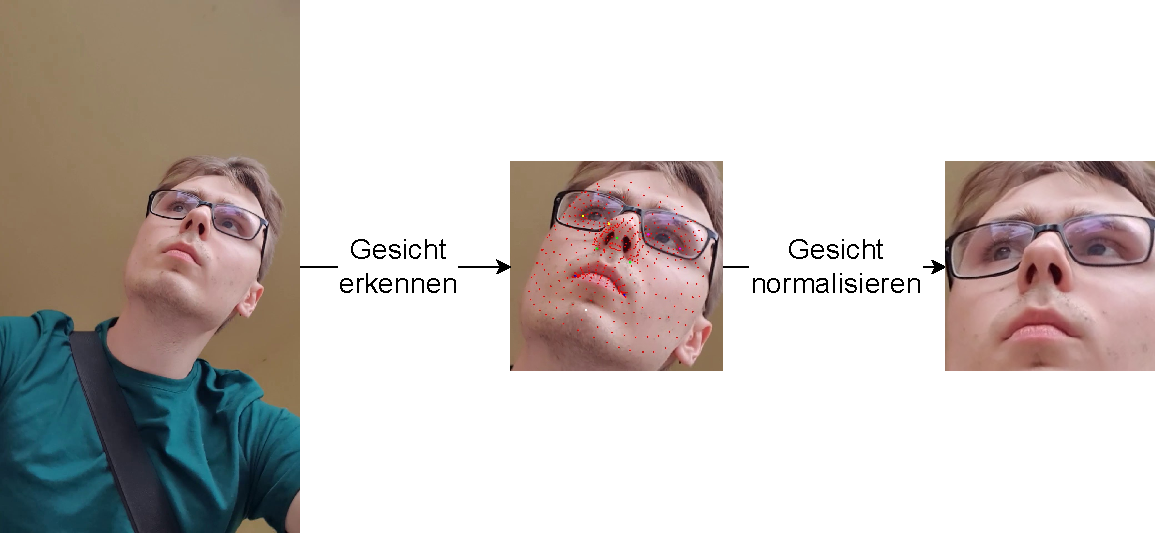
\includegraphics[width=\linewidth]{concept/normalisierung.drawio.pdf}
\caption{Beispielhafte Darstellung eines normalisierten Gesichts.}
\label{fig:concept:normalisation}
\end{figure}

Aus dem normalisierten Bild wird dann die Blickrichtung mithilfe von Convolutional Neural Networks vorhergesagt, die auf dem \textit{ETH-XGaze} \cite{paper:eth-xgaze}, \textit{Gaze360} \cite{paper:gaze360} und dem \textit{MPIIFaceGaze} \cite{paper:mpiifacegaze} Datensatz trainiert wurden. Das Ergebnis beschreibt dann die Blickrichtung des normalisierten Gesichts. Es muss daher wieder in das Koordinatensystem vor der Normalisierung transformiert werden, um die tatsächliche Blickrichtung $\gazevector$ zu erhalten. Mit dem Vektor $\gazevector$ wird dann zusammen mit der dreidimensionalen Position des Kopfes $\centerface$ eine Gerade $G$ entlang der Blickrichtung konstruiert. Mit $G$ wird dann der Schnittpunkt $\intersection$ mit der Ebene $\cameraplane$ bestimmt.  

Die Ergebnisse dieses Konzepts sollen dann genauso wie die Ergebnisse des Konzepts zur Bestimmung der Blickrichtung mittels der Kopfrotation evaluiert werden. Dafür wird für die entstandenen Schnittpunkte untersucht, bei welchen dieser Schnittpunkte die Person auf das Smartphone sieht, um so eine Zone auf der Ebene $\cameraplane$ zu bestimmen, die das Display des Smartphones repräsentiert (siehe Abbildung \ref{fig:concept:head:example}).

Bei vielen der im Kapitel \ref{sec:related:gaze} vorgestellten Datensätze wurden Bilder mit geschlossenen Augen bei der Datensatzerstellung aussortiert \cite{paper:eth-xgaze, paper:rt_gene, paper:tabletgaze}. Daher sollen auch in dieser Arbeit Bilder mit geschlossenen Augen identifiziert werden, um diese bei der Interpretation der Blickrichtung zu ignorieren.

Einen möglichen Ansatz für die Erkennung von geschlossenen Augen stellen Ibrahim et al. in ihrer Arbeit \cite{paper:ear} vor. Sie verwenden erkannte Gesichtspunkte rund um das Auge, um zu bestimmen, ob ein Auge offen (siehe Abbildung \ref{fig:concept:ear:open}) oder geschlossen (siehe Abbildung \ref{fig:concept:ear:closed}) ist. 

\begin{figure}[]
    \begin{subfigure}{0.45\textwidth}
        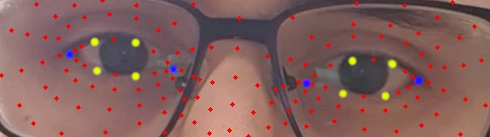
\includegraphics[width=\linewidth]{concept/ear-augen-offen.jpg}
        \caption{Augen geöffnet}
        \label{fig:concept:ear:open}
    \end{subfigure}%
    \vspace{0.5cm}
    \begin{subfigure}{0.45\textwidth}
        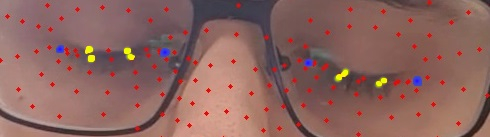
\includegraphics[width=\linewidth]{concept/ear-augen-zu.jpg}
        \caption{Augen geschlossen}
        \label{fig:concept:ear:closed}
    \end{subfigure}
    \begin{subfigure}{0.45\textwidth}
        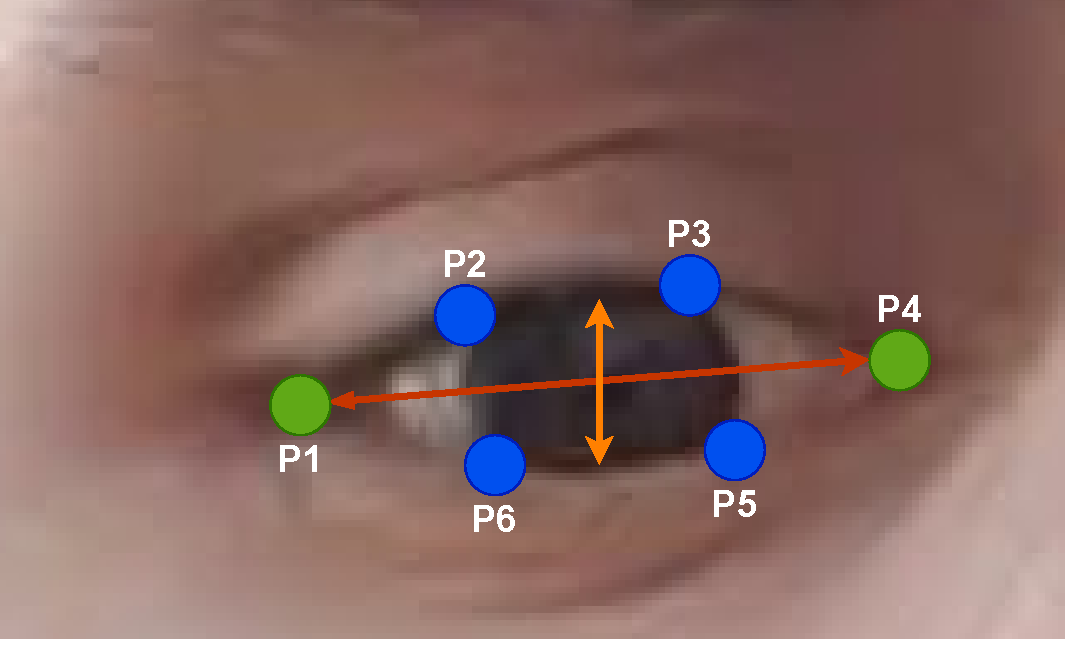
\includegraphics[width=\linewidth]{implementation/ear.drawio.pdf}
        \caption{Benötigte Punkte für die Berechnung des $EAR$}
        \label{fig:concept:ear:points}
    \end{subfigure}
    \caption{Erkennung von geschlossenen Augen anhand augenbezogener Gesichtspunkte.}
    \label{fig:concept:ear}
\end{figure}

Dazu wird das \textit{Eye Aspect Ratio} ($\ear$) berechnet. Dieser Wert errechnet sich aus sechs Punkten $P_1$ bis $P_6$ um das Auge herum. Die benötigten Punkte sind in Abbildung \ref{fig:concept:ear:points} dargestellt. Der Wert wird zunächst für jedes Auge einzeln mit folgender Formel berechnet:

\[
EAR_{\text{links/rechts}} = \frac{\|P_2 - P_6\| + \|P_3 - P_5\|}{2\|P_1 - P_4\|}
\]

Anschließend wird der Mittelwert aus beiden Werten gebildet. Dieser ergibt dann den endgültigen $EAR$-Wert.

\[
EAR = \frac{EAR_{\text{links}} + EAR_{\text{rechts}}}{2}
\]

Um nun zu entscheiden, ob eine Auge offen oder geschlossen ist, muss ein Grenzwert $\earthreshold$ festgelegt werden. Ist der berechnete Wert größer als $\earthreshold$, dann sind die Augen geöffnet. Wenn der Wert kleiner ist, sind die Augen geschlossen. Der ideale Grenzwert soll dabei während der Evaluation bestimmt werden.

\section{Zusammenfassung}

In diesem Kapitel wurden drei verschiedene Ansätze zur Bestimmung der Blickrichtung von Radfahrenden untersucht. 

Dabei hat sich gezeigt, dass Modelle, die für die Vorhersage von zweidimensionalen Bildschirmkoordinaten trainiert wurden, für die Anwendung im Rahmen der PrioBike-App nicht geeignet sind, da keine Aussage über die Blickrichtung der Radfahrenden getroffen werden kann, wenn diese nicht auf das Smartphone-Display schauen.

Weiter wurde untersucht, wie die Bestimmung der Blickrichtung anhand der Kopfrotation sowie mittels Convolutional Neural Networks in die PrioBike-App integriert werden kann. Dabei wurden zwei Konzepte entwickelt. In beiden Konzepten werden Radfahrende während der Fahrt mit der Innenkamera des Smartphones am Lenker gefilmt. Für die einzelnen Bilder dieser Videos wird anschließend eine Gesichtserkennung durchgeführt. Diese besteht aus dem Erkennen der Bounding Box des Gesichts, der Bestimmung von Gesichtspunkten in Form von zweidimensionalen Bildkoordinaten sowie der Bestimmung von der dreidimensionalen Position des Gesicht relativ zur Kamera.

Darauf aufbauend wird eine dreidimensionale Blickrichtung mit den beiden Konzepten auf unterschiedliche Weise bestimmt. Im ersten Konzept wird die dreidimensionale Drehung des Kopfes verwendet, um einen Vektor $\gazevector$ zu konstruieren, der die Blickrichtung der abgebildeten Person repräsentiert. Im zweiten Konzept werden Convolutional Neural Networks verwendet, um den Vektor $\gazevector$ zu bestimmen. Die Convolutional Neural Networks werden mit drei verschiedenen Datensätzen trainiert. Diese Datensätze sind \ethg \cite{paper:eth-xgaze}, \gazed \cite{paper:gaze360} und \mpii \cite{paper:mpiifacegaze}. 

Mithilfe des Vektors $\gazevector$ und der dreidimensionalen Position des Kopfes wird dann eine Gerade $G$ definiert. Mit $G$ wird ein Schnittpunkt $\intersection$ mit der Ebene $\cameraplane$ berechnet. Während der Auswertung wird untersucht, bei welchem dieser Schnittpunkte die Person auf das Smartphone geschaut hat, um einen Bereich auf der Ebene $\cameraplane$ zu definieren, der ein virtuelles Smartphone darstellt. Liegt ein Schnittpunkt $\intersection$ innerhalb dieses Bereichs, so hat die Person auf das Smartphone gesehen. Die Erkennung der Blickrichtung basiert auf den Ergebnissen der Gesichtserkennung. Wird kein Gesicht erkannt, kann der Vektor $\gazevector$ nicht bestimmt werden. Es wird davon ausgegangen, dass in den meisten Fällen ein nicht erkanntes Gesicht auf eine Drehung des Kopfes entlang der Querachse zurückzuführen ist. Da sich das Smartphone in diesem Fall nicht im Blickfeld der Person befindet, wird angenommen, dass die Person nicht auf das Smartphone schaut, wenn kein Gesicht erkannt wurde. Diese Annahme wird in der Evaluation überprüft.













